\chapter{Prototipação}
\label{apendice_e}
A prototipação validou o uso do mini-projetor UC46. Este possui uma potência de 1200 lumens, e havia preocupação quanto à qualidade da imagem gerada. O teste ocorreu em uma sala de 25 metros quadrados, com uma lâmpada de LED, de 7W e luminosidade de 7 lumens, e uma janela parcialmente aberta (Figura \ref{fig:projection}). A incidência de luz externa (porta aberta) sobre a projeção prejudicou a qualidade da imagem, porém com a porta fechada o contraste obtido viabilizou a continuidade do projeto.
% preocupação com luminosidade
\begin{figure*}[h]
    \centering
    \begin{subfigure}{.33\textwidth}
        \centering
        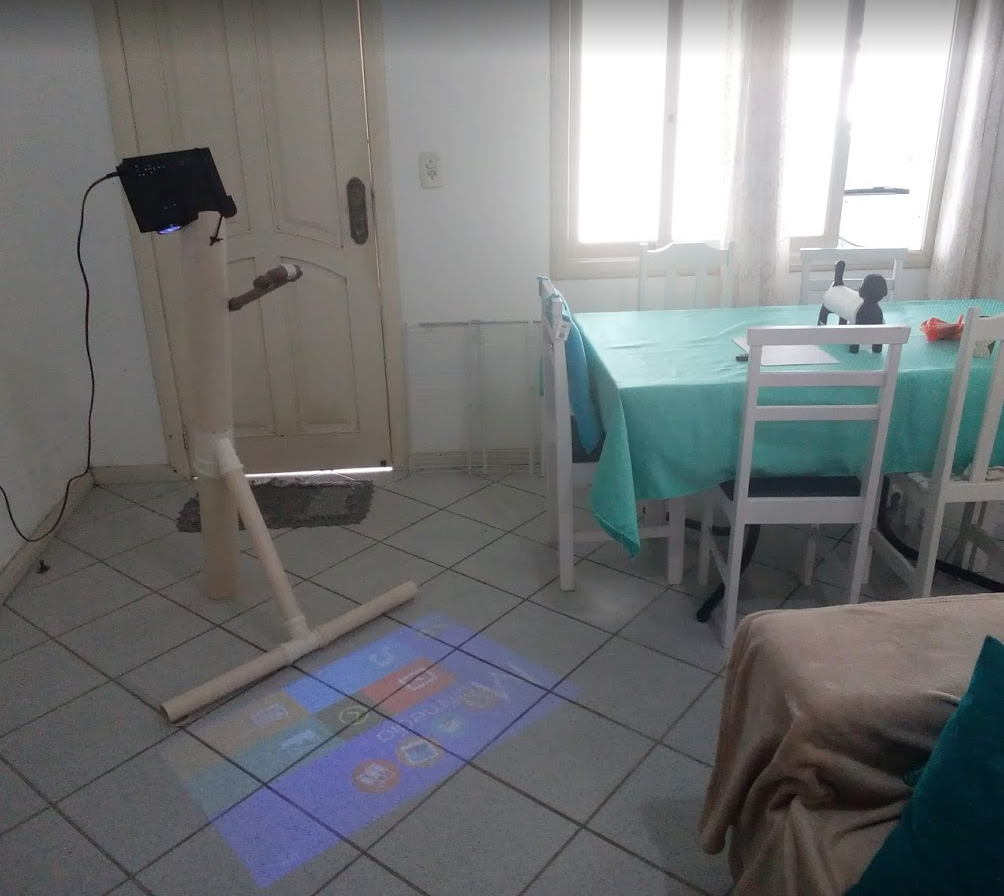
\includegraphics[width=.9\linewidth,fbox]{figs/projection.png}
        \caption{Projeção em ambiente iluminado por lâmpada de 700 lumens}
        \label{fig:projection}
    \end{subfigure}%
    \begin{subfigure}{.33\textwidth}
        \centering
        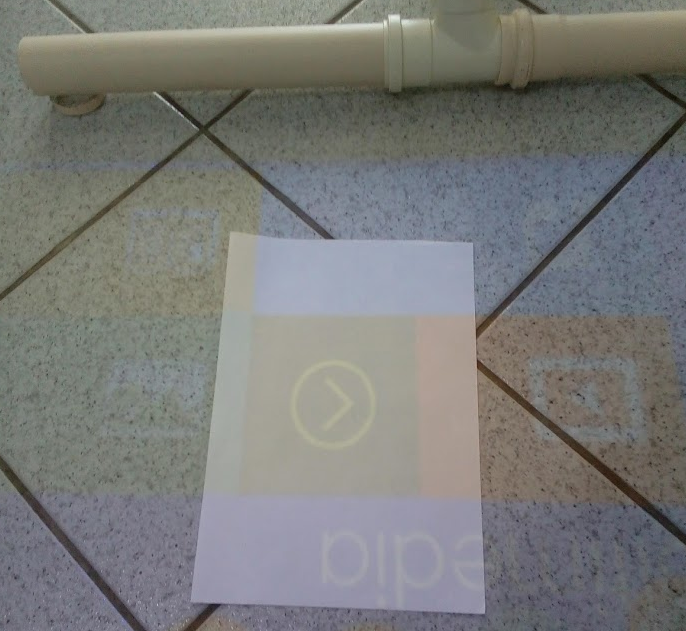
\includegraphics[width=.9\linewidth,fbox]{figs/projection_day.png}
        \caption{Projeção com a incidência de luz externa}
        \label{fig:projection_day}
    \end{subfigure}%
    \begin{subfigure}{.33\textwidth}
        \centering
        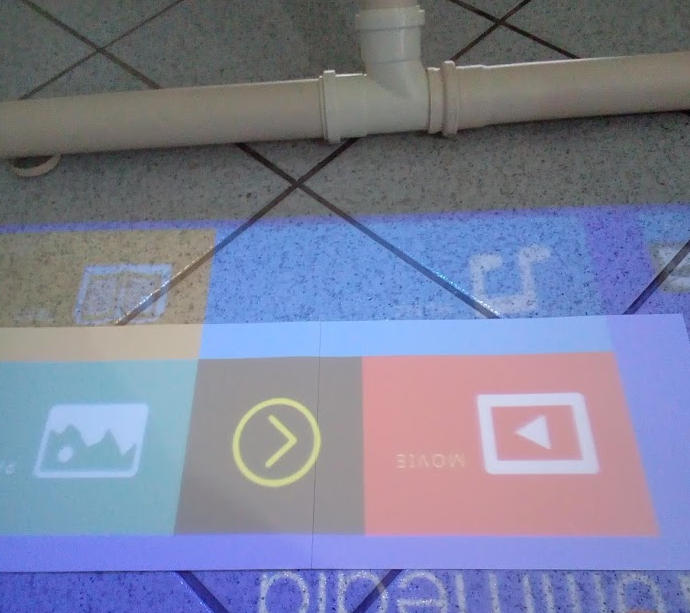
\includegraphics[width=.9\linewidth,fbox]{figs/projection_night.png}
        \caption{Projeção sem incidência de luz externa}
        \label{fig:projection_night}
    \end{subfigure}%
    \caption{Qualidade da projeção em diferentes condições luminosas.}
    \sourceauthor
    \label{fig:proj_light}
\end{figure*}
% estrutura de pvc
A estrutura para posicionar o projetor usa PVC e não utiliza cola, para permitir reprodução. O projeto da estrutura foi feito em 3D e busco eliminar ao máximo o uso de materiais. A rigidez da estrutura também foi testada para verificar se não cairia para os lados.
% correção do posicionamento

A prototipação também permitiu corrigir o posicionamento da imagem captada pela câmera. Devido à inclinação entre a câmera e a superfície de projeção, a visão da câmera fica em perspectiva. Porém essa perspectiva precisa ser eliminada para encontrar a posição correta dos blocos no mapa (Figura \ref{fig:homography}). Isso é feito criando uma matriz homográfica \cite{dubrofsky_homography_2009}. 

\begin{figure*}[!htpb]
    \centering
    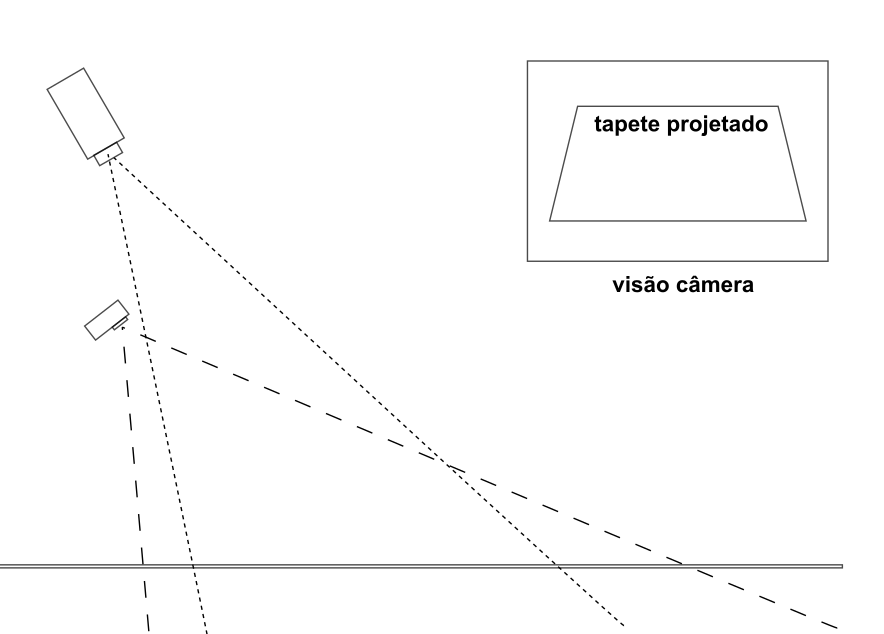
\includegraphics[width=0.7\textwidth, fbox]{figs/homography.png}
    \caption{Inclinação entre câmera, projetor e superfície.}
    \label{fig:homography}
\end{figure*}

Protótipos dos blocos de papelão (Figura \ref{fig:paper_blocks}) produzidos tem cores correspondentes às cores dos botões do brinquedo RoPE. O tamanho é 7,5x10cm e o diâmetro da marca fiducial é 2,5cm, de modo que a câmera reconhece os blocos a 100cm de distância. Posteriormente o diâmetro foi aumentado para 4cm.

\begin{figure*}[!htpb]
    \centering
    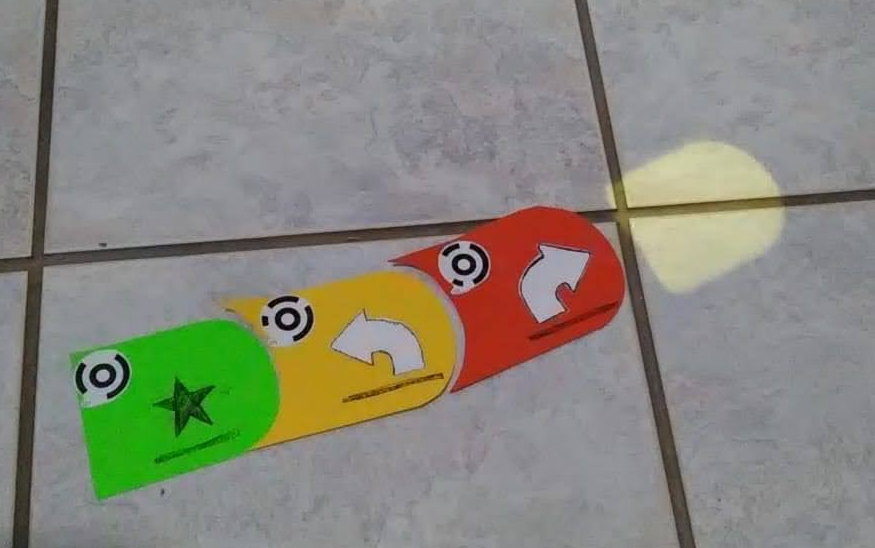
\includegraphics[width=0.7\textwidth, fbox]{figs/paper_blocks.png}
    \caption{Blocos de papel e projeção de um indicador para o local do próximo bloco.}
    \label{fig:paper_blocks}
\end{figure*}